\section{Further Examples of Metric Spaces}

The $l^p$ proof is a bit annoying, I had to read through it carefully to really get it.

We have $p \in \R$, and $x = (\xi_j) = (\xi_1, \xi_2, \dots)$ such that

\begin{equation}
  \sum_{j=1}^\infty |\xi_j|^p < \infty. \tag{$p\geq 1$}
\end{equation}

and the metric is defined by

\begin{equation}
  d(x, y) = \pa{\sum_{j=1}^\infty |\xi_j - \eta_j|^p}^{1/p}.
\end{equation}

For $p= 2$, we have the Hilbert space $l^2$.

We now want to prove that $l^p$ is a metric space.

\begin{proof}
  Properties 1-3 are pretty straightforward, so we really just need to show convergence and the triangle inequality.

  We are starting with a auxiliary inequality
  \begin{equation}
    \frac{1}{p} + \frac{1}{q} = 1
  \end{equation}

  From this inequality, where $p, q$ are \textbf{conjugate exponents}, we can derive $1/(p-1) = q - 1$. Therefore, we can say
  \begin{equation}
    u = t^{p-1} \implies t = u^{1/(p-1)} = u^{q-1}.
  \end{equation}

  Now, suppose $\alpha, \beta \geq 0$. Since $\alpha\beta$ is the area of a rectangle in \ref{fig:youngs_inequality}, we can bound it above by the integral curves.
  The intuition here is, we want to consider the area under the curve, vertically and horizontally. We have 3 cases:
  \begin{enumerate}
    \item If the corner $(\alpha, \beta)$ is exactly at the corner of the rectangle, then the rectangle area is exactly the sum of the two areas.
    \item If the end of the curve at $\alpha$ is above $\beta$, then the rectangle is smaller than the sum of the two areas, because the curve has more area above the $\beta$ line.
    \item If the end of the curve at $\alpha$ is below $\beta$, then the rectangle is still smaller than the sum of the two areas, since it has more horizontal area past $\alpha$.
  \end{enumerate}

  \begin{figure}[H]
    \centering
    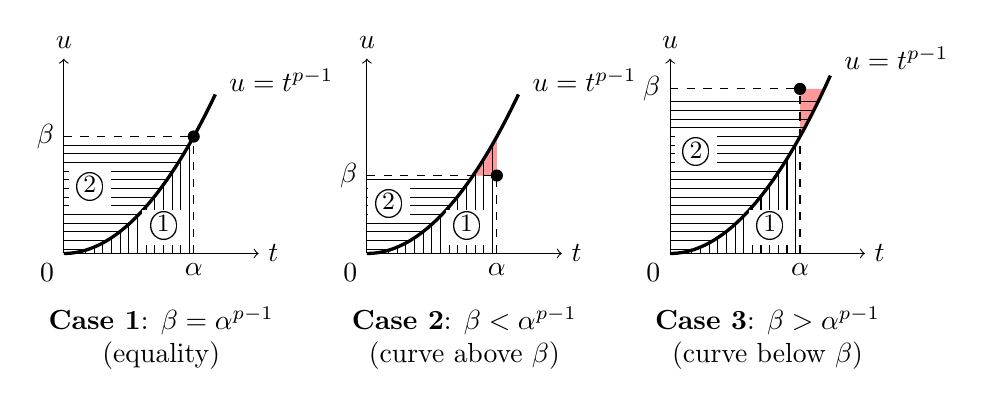
\begin{tikzpicture}[scale=0.55]
      % Case 1: Equality - corner exactly on curve
      \begin{scope}
        % Axes
        \draw[->] (0,0) -- (4.5,0) node[right] {$t$};
        \draw[->] (0,0) -- (0,4.5) node[above] {$u$};
        \node[below left] at (0,0) {$0$};

        % For equality: beta = alpha^{p-1} (corner on curve)
        \def\alph{3}
        \pgfmathsetmacro{\bet}{0.3*\alph*\alph} % beta = 2.7

        % Region 1 - vertical lines (area under curve from 0 to alpha)
        \foreach \x in {0.1,0.3,...,2.9} {
          \pgfmathsetmacro{\yval}{0.3*\x*\x}
          \draw[thin] (\x,0) -- (\x,\yval);
        }

        % Region 2 - horizontal lines (area to left of curve from 0 to beta)
        \foreach \y in {0.1,0.3,...,2.5} {
          \pgfmathsetmacro{\xval}{sqrt(\y/0.3)}
          \draw[thin] (0,\y) -- (\xval,\y);
        }

        % The curve u = t^{p-1}
        \draw[very thick, domain=0:3.5, samples=100] plot (\x, {0.3*\x*\x});

        % Rectangle boundary - corner ON the curve
        \draw[dashed] (\alph,0) -- (\alph,\bet);
        \draw[dashed] (0,\bet) -- (\alph,\bet);
        \fill (\alph,\bet) circle (4pt); % Mark the corner point

        % Labels
        \node[below] at (\alph,0) {$\alpha$};
        \node[left] at (0,\bet) {$\beta$};
        \node[fill=white, inner sep=2pt] at (2.3,0.6) {\textcircled{\small 1}};
        \node[fill=white, inner sep=2pt] at (0.6,1.5) {\textcircled{\small 2}};
        \node[right] at (3.6,4) {$u = t^{p-1}$};
        \node[below, align=center] at (2.25,-1) {\textbf{Case 1}: $\beta = \alpha^{p-1}$\\(equality)};
      \end{scope}

      % Case 2: Curve at alpha is ABOVE beta
      \begin{scope}[xshift=7cm]
        % Axes
        \draw[->] (0,0) -- (4.5,0) node[right] {$t$};
        \draw[->] (0,0) -- (0,4.5) node[above] {$u$};
        \node[below left] at (0,0) {$0$};

        % beta < alpha^{p-1} (curve goes above beta at alpha)
        \def\alph{3}
        \def\bet{1.8} % Below curve value of 2.7
        \pgfmathsetmacro{\curveatalpha}{0.3*\alph*\alph}

        % Extra sliver in RED - area between beta and curve (above rectangle)
        \fill[red!40] plot[domain={sqrt(\bet/0.3)}:\alph, samples=50] (\x, {0.3*\x*\x}) -- (\alph,\bet) -- ({sqrt(\bet/0.3)},\bet) -- cycle;

        % Region 1 - vertical lines (area under curve from 0 to alpha)
        \foreach \x in {0.1,0.3,...,2.9} {
          \pgfmathsetmacro{\yval}{0.3*\x*\x}
          \draw[thin] (\x,0) -- (\x,\yval);
        }

        % Region 2 - horizontal lines (area to left of curve from 0 to beta)
        \foreach \y in {0.1,0.3,...,1.7} {
          \pgfmathsetmacro{\xval}{sqrt(\y/0.3)}
          \draw[thin] (0,\y) -- (\xval,\y);
        }

        % The curve u = t^{p-1}
        \draw[very thick, domain=0:3.5, samples=100] plot (\x, {0.3*\x*\x});

        % Rectangle boundary - corner BELOW the curve
        \draw[dashed] (\alph,0) -- (\alph,\bet);
        \draw[dashed] (0,\bet) -- (\alph,\bet);
        \fill (\alph,\bet) circle (4pt); % Mark the corner point

        % Labels
        \node[below] at (\alph,0) {$\alpha$};
        \node[left] at (0,\bet) {$\beta$};
        \node[fill=white, inner sep=2pt] at (2.3,0.6) {\textcircled{\small 1}};
        \node[fill=white, inner sep=2pt] at (0.5,1.1) {\textcircled{\small 2}};
        \node[right] at (3.6,4) {$u = t^{p-1}$};
        \node[below, align=center] at (2.25,-1) {\textbf{Case 2}: $\beta < \alpha^{p-1}$\\(curve above $\beta$)};
      \end{scope}

      % Case 3: Curve at alpha is BELOW beta
      \begin{scope}[xshift=14cm]
        % Axes
        \draw[->] (0,0) -- (4.5,0) node[right] {$t$};
        \draw[->] (0,0) -- (0,4.5) node[above] {$u$};
        \node[below left] at (0,0) {$0$};

        % beta > alpha^{p-1} (curve goes below beta at alpha)
        \def\alph{3}
        \def\bet{3.8} % Above curve value of 2.7
        \pgfmathsetmacro{\curveatalpha}{0.3*\alph*\alph}

        % Extra sliver in RED - area between alpha and curve (past rectangle horizontally)
        \fill[red!40] plot[domain=\alph:{sqrt(\bet/0.3)}, samples=50] (\x, {0.3*\x*\x}) -- ({sqrt(\bet/0.3)},\bet) -- (\alph,\bet) -- (\alph,\curveatalpha) -- cycle;

        % Region 1 - vertical lines (area under curve from 0 to alpha)
        \foreach \x in {0.1,0.3,...,2.9} {
          \pgfmathsetmacro{\yval}{0.3*\x*\x}
          \draw[thin] (\x,0) -- (\x,\yval);
        }

        % Region 2 - horizontal lines (area to left of curve from 0 to beta)
        \foreach \y in {0.1,0.3,...,3.6} {
          \pgfmathsetmacro{\xval}{sqrt(\y/0.3)}
          \draw[thin] (0,\y) -- (\xval,\y);
        }

        % The curve u = t^{p-1}
        \draw[very thick, domain=0:3.7, samples=100] plot (\x, {0.3*\x*\x});

        % Rectangle boundary - corner ABOVE the curve
        \draw[dashed] (\alph,0) -- (\alph,\bet);
        \draw[dashed] (0,\bet) -- (\alph,\bet);
        \fill (\alph,\bet) circle (4pt); % Mark the corner point

        % Labels
        \node[below] at (\alph,0) {$\alpha$};
        \node[left] at (0,\bet) {$\beta$};
        \node[fill=white, inner sep=2pt] at (2.3,0.6) {\textcircled{\small 1}};
        \node[fill=white, inner sep=2pt] at (0.6,2.3) {\textcircled{\small 2}};
        \node[right] at (3.8,4.5) {$u = t^{p-1}$};
        \node[below, align=center] at (2.25,-1) {\textbf{Case 3}: $\beta > \alpha^{p-1}$\\(curve below $\beta$)};
      \end{scope}
    \end{tikzpicture}
    \caption{Integral inequality cases. The red areas are the excess}
    \label{fig:youngs_inequality}
  \end{figure}

  The diagrams in \ref{fig:youngs_inequality} illustrate these cases. Now, we can derive

  \begin{equation}
    \alpha\beta \leq \int_0^\alpha t^{p-1} \dd{t} + \int_0^\beta u^{q-1} \dd{u} = \frac{\alpha^p}{p} + \frac{\beta^q}{q}.
    \label{eq:youngs_inequality}
  \end{equation}

  Now, suppose we have sequences $(\xi_j), (\eta_j)$, such that
  \begin{equation}
    \sum_{j=1}^\infty |\xi_j|^p = 1, \quad \sum_{j=1}^\infty |\eta_j|^q = 1.
  \end{equation}
  From \eqref{eq:youngs_inequality}, and summing over $j$, we have
  \begin{equation}
    \sum_{j=1}^\infty |\xi_j \eta_j| \leq \sum_{j=1}^\infty \pa{\frac{|\xi_j|^p}{p} + \frac{|\eta_j|^q}{q}} =
    \frac{1}{p} + \frac{1}{q} = 1.
    \label{eq:normalized_holder}
  \end{equation}
  Now, if we want to choose any arbitrary sequences $(\xi_j), (\eta_j)$, we can normalize them by defining
  \begin{equation}
    \tilde{\xi_j} = \frac{\xi_j}{\pa{\sum_{k=1}^\infty |\xi_k|^p}^{1/p}},
    \quad \tilde{\eta_j} = \frac{\eta_j}{\pa{\sum_{k=1}^\infty |\eta_k|^q}^{1/q}},
  \end{equation}
  and we can now substitute into \eqref{eq:normalized_holder} to get
  \begin{align*}
    \sum_{j=1}^\infty |\xi_j \eta_j| &\leq 1\\
    \sum_{j=1}^\infty \abs{
      \frac{\xi_j}{\pa{\sum_{k=1}^\infty |\xi_k|^p}^{1/p}} \cdot
      \frac{\eta_j}{\pa{\sum_{k=1}^\infty |\eta_k|^q}^{1/q}}
    } &\leq 1 \tag{Substitute normalizations}\\
    \sum_{j=1}^\infty |\xi_j \eta_j| &\leq
    \pa{\sum_{k=1}^\infty |\xi_k|^p}^{1/p}
    \pa{\sum_{k=1}^\infty |\eta_k|^q}^{1/q}.
  \end{align*}
  This now gives us \textbf{Hölder's inequality}.

  We now need to prove \textbf{Minkoswki's inequality}, which is the triangle inequality for $l^p$.
  We start by using $\omega_j = \xi_j + \eta_j$. Then, what we can do is use the triangle inequality to get
  \begin{align*}
    \abs{\omega_j} &\leq \abs{\xi_j + \eta_j}\\
    \abs{\omega_j}^p &\leq \abs{\xi_j + \eta_j}\abs{\omega_j}^{p-1} \\
    \abs{\omega_j}^p &\leq \pa{\abs{\xi_j} + \abs{\eta_j}}\abs{\omega_j}^{p-1} \tag{Triangle inequality}\\
    \sum\abs{\omega_j}^p &\leq \sum \abs{\xi_j}\abs{\omega_j}^{p-1} + \sum\abs{\eta_j}\abs{\omega_j}^{p-1} \tag{Applying sum}\\
  \end{align*}
  Now we can apply Hölder's inequality to each of the sums on the right-hand side, where we have conjugate exponents $p$ and $q$, which gives us:
  \begin{align*}
    \sum\abs{\omega_j}^p
    &\leq
    \pa{
      \sum \abs{\xi_j}^p
    }^{1/p}
    \pa{
      \sum \abs{\omega_j}^{(p-1)q}
    }^{1/q}
    +
    \pa{
      \sum \abs{\eta_j}^p
    }^{1/p}
    \pa{
      \sum \abs{\omega_j}^{(p-1)q}
    }^{1/q}\\
    &\leq
    \pa{
      \sum \abs{\xi_j}^p
    }^{1/p}
    \pa{
      \sum \abs{\omega_j}^p
    }^{1/q}
    +
    \pa{
      \sum \abs{\eta_j}^p
    }^{1/p}
    \pa{
      \sum \abs{\omega_j}^p
    }^{1/q} \tag{Since $(p-1)q = p$}\\
    &\leq
    \pbra{
      \pa{
        \sum \abs{\xi_j}^p
      }^{1/p}
      +
      \pa{
        \sum \abs{\eta_j}^p
      }^{1/p}
    }
    \pa{
      \sum \abs{\omega_j}^p
    }^{1/q}
  \end{align*}
  Finally, dividing both sides by $\pa{\sum \abs{\omega_j}^p}^{1/q}$:
  \begin{align*}
    \pa{\sum \abs{\omega_j}^p}^{1 - 1/q}
    &\leq
    \pa{\sum \abs{\xi_j}^p}^{1/p}
    +
    \pa{\sum \abs{\eta_j}^p}^{1/p}
  \end{align*}
  Since $1 - \frac{1}{q} = \frac{1}{p}$ (from $\frac{1}{p} + \frac{1}{q} = 1$), we have
  \begin{equation}
    \pa{\sum \abs{\xi_j + \eta_j}^p}^{1/p}
    \leq
    \pa{\sum \abs{\xi_j}^p}^{1/p}
    +
    \pa{\sum \abs{\eta_j}^p}^{1/p}
  \end{equation}
  which is \textbf{Minkowski's inequality}.

  Finally, we need to show the triangle inequality for the metric.

  We take $x = (\xi_j), y = (\eta_j), z = (\zeta_j)$, and we have
  \begin{align*}
    d(x, z) &= \pa{\sum |\xi_j - \zeta_j|^p}^{1/p} \\
    &= \pa{\sum |\xi_j - \eta_j + \eta_j - \zeta_j|^p}^{1/p} \\
    &\leq \pa{\sum |\xi_j - \eta_j|^p}^{1/p} + \pa{\sum |\eta_j - \zeta_j|^p}^{1/p} \tag{Minkowski's inequality}\\
    &= d(x, y) + d(y, z).
  \end{align*}
  This completes the proof that $l^p$ is a metric space.
\end{proof}